\chapter{Aktuelle Engineentwicklung}
\label{chap:engine-uebersicht}

%% Zitat:
% https://twitter.com/CompSciFact/status/527816734863265792
\epigraph{"`Even if your code was perfect when you released it, it still needs to be maintained because the world around it is changing."'}{Unbekannt}

Spiele- und Grafikengines sind inzwischen äußerst komplexe Softwareprojekte. Früher wurden Spiele von Einzelpersonen oder kleinen Teams entwickelt, heute sind Teamstärken von über 100 Entwicklern aus unterschiedlichen Disziplinen keine Seltenheit. Komplexe Softwareprojekte erfordern neue Projektstrukturen, und dementsprechend haben sich die Projektstrukturen aber auch die Organisationformen der Teams im Laufe der Zeit gewandelt.

Mit der Professionalisierung der Branche sind auch die Anforderungen an die Software zumindest inzwischen klar definiert: Das Softwareprojekt ist langfristing angelegt (Spiele-Engines auf Jahrzente), soll dem entsprechend robust und flexibel, wartbar, zugänglich und angemessen verständlich sein. Projektstrukturen sind inzwischen häufig auf kurze Iterationszyklen ausgelegt. Durch die kurzen Iterationszyklen werden konkrete Ziele in Reichweite gesteckt, damit sich das Erreichen oder Nichterreichen zeitnah abschätzen lässt. Weiter sollen kurze Iterationszyklen dem Entwicklerteam ermöglichen, auf die verändernde Umwelt zu reagieren und sich neuen Anforderungen flexibel anzupassen.

Im letzten Jahr hat sich der Markt der kommerziellen Spiele- und Grafik-Engines sehr verändert. Die wichtigsten Entwickler von kommerziellen Engines, wie \textit{Epic Games} oder \textit{Crytek}, haben ihre Projekte der Allgemeinheit gegenüber geöffnet, während früher noch sechsstellige Beträge für den Einblick in den Quelltext zu zahlen waren. Inzwischen rufen die Entwickler direkt zur Mitarbeit an ihrer Engine auf. Das bringt für beide Seiten Vorteile. Zwar muss der beitragende Entwickler auf seine Rechte am Code verzichten\footnote{Abschnitt 8. 8. Feedback and Contributions: https://www.unrealengine.com/eula}, doch kann er direkten Einfluss auf die Entwicklung kommerzieller Schlüsselsoftware nehmen. Und auf der anderen Seite kann das Unternehmen den Eifer der Entwickler kommerziell verwerten aber auch neue fähige Mitarbeiter sichten und gegebenfalls rekrutieren.

Zusätzlich hat sich der Fokus der aktuellen Engines deutlich verschoben. Während vor ein paar Jahren die Editoren komplex zu bedienen waren und tiefergehende Programmierkenntnisse benötigt wurden, sind die aktuellen Editoren deutlich einsteigerfreundlicher geworden. Erste Prototypen oder einfache Spiele sind in Editoren wie dem \textit{Unreal Editor} über das \textit{Blueprint} genannte System ohne eigentliche Programmierkenntnisse umsetzbar. Werden komplexere und spezifische Blueprints benötigt, können \textit{Blueprints} in C++ umgesetzt werden.

\begin{figure}
\centering
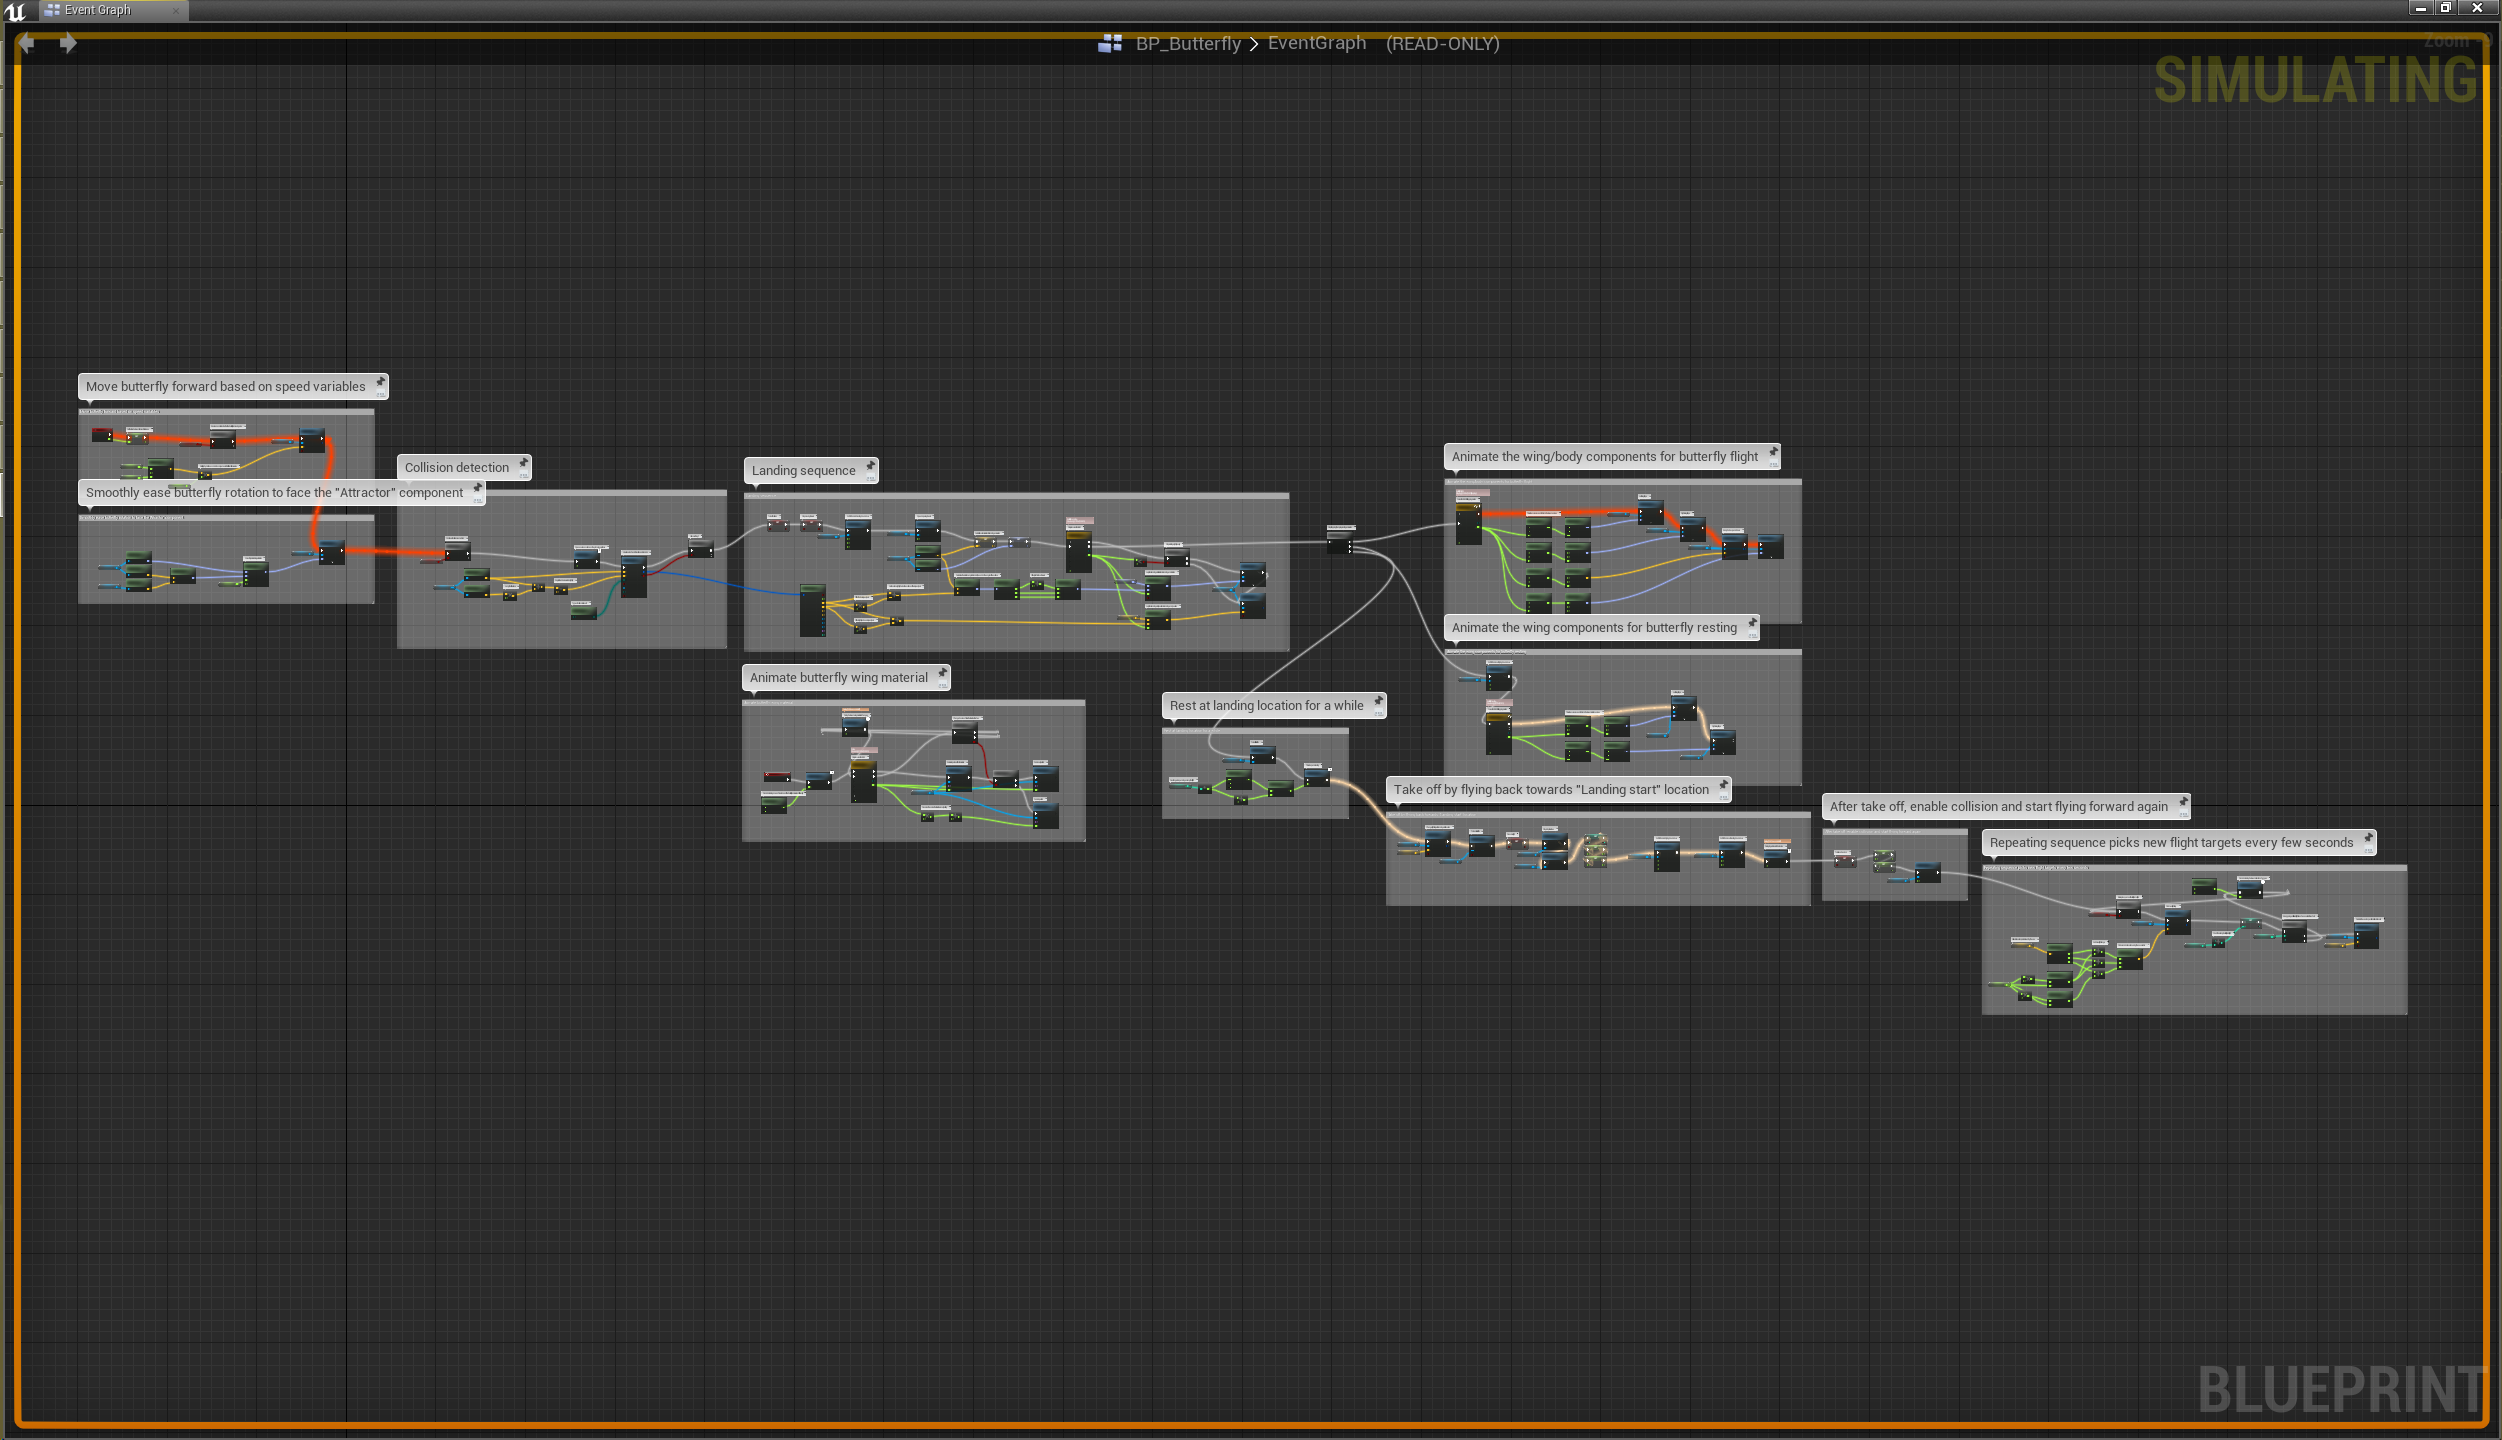
\includegraphics[width=\textwidth]{ue4-blueprint}
\caption{Unreal Engine 4 Blueprint Beispiel}
\end{figure}

\section{Grafik-Engines in Haskell}

C bzw. C++ ist quasi der Industriestandard in der Grafik- und Spieleprogrammierung. Doch gibt es auch einige Open-Source Engines die in anderen Sprachen implementiert wurden. Die folgende Betrachtung beschränkt sich auf Engines die entweder direkt in Haskell umgesetzt wurden oder die auf Bindings zu bestehenden Open-Source Engines basieren.

\subsection{HGamer3D}

\textit{HGamer3D}\footnote{http://www.hgamer3d.org/} basiert auf (nich kompletten) Haskell-Bindings zu \textit{Ogre}\footnote{http://www.ogre3d.org/}. Ogre ist eine objektorientierte Open-Source Grafik-Engine geschrieben in C++. Ohne weiter auf die Fähigkeiten der Ogre Engine einzugehen, stellt sich oft die Adaptierunung von imperativen Bibliotheken auf funktionale Konzepte als aufwändig und nicht immer optimal heraus. Insbesondere dass die Haskell-Bindings zu komplexen C++ \acsp{API} größtenteils von Hand erzeugt werden müssen, setzt immer noch hohe Hürden.

Auch wenn Ogre als Framework viele Strukturen und Lösungsansätze für gängige Probleme in der 3D Computergrafik und Spieleprogrammierung bereitstellt, ließen sich viele Ansätze auch direkt funktional umsetzen, ohne große und schwerfällige \acsp{API} adaptieren zu müssen.

Zum Beispiel verfolgen beide Welten zum Teil gänzlich andere Grundprinzipien. So sind Daten in Haskell prinzipiell unveränderlich während in C++ Daten prinzipiell veränderlich sind. Haskell erlaubt unter anderem deswegen andere Ansätze der Nebenläufigkeit (Concurrency). Speziell Nebenläufigkeiten stellen immer noch in komplexen Softwareprojekten eine große Hürde dar. Die Adaption einer C++-Biblithek kann das Ausnutzen vieler Vorteile von Haskell behindern (weitere Ausführungen in \fref{sec:warum-haskell}).

Zusätzlich entstehen durch Bindings zu externen Bibliotheken neue Abhängigkeiten, die oft eine Anpassung der Tool-Chain erfordern, da sie nicht in das bestehende Ökosystem passen. Dies erhöht die Komplexität des Gesamtsystems. Die Erfahrung des Autors hat gezeigt, dass externe Bindings oft zu Komplikationen führen, spätestens dann, wenn die Anwendung die Entwicklungsumgebung verlässt. In der Praxis lassen sich aber selten Abhhängigkeiten zu anderen Sprachen komplett vermeiden. Insbesondere in der Grafikprogrammierung mit \textit{OpenGL} werden die eigentlichen Bindings zu der \textit{OpenGL}-API benötigt. Zusätzlich muss noch ein plattformabhängiger Render-Kontext erzeugt werden. Dessen Erzeugung ist nicht Teil von \textit{OpenGL} und erfordert eine weitere externe Komponente.

Meinung des Autors: Es sollten möglichst wenige Fremdabhängigkeiten aus anderen Sprachen genutzt werden, leider ist dies nicht immer möglich (Weitere Ausführungen in \fref{sec:probleme-haskell}). Mit den Ogre Bindings wird die eine komplexe schwer funktional bezwingbare \acs{API} (z.B. \textit{OpenGL}) mit einer anderen ersetzt. Vorteil ist unbestritten, dass die Engine ausgereift ist und vieles nicht erst neu implementiert werden muss.

\subsection{LambdaCube 3D}

\textit{LambdaCube 3D}\footnote{https://lambdacube3d.wordpress.com/} ist eine in Haskell definierte und mächtige \ac{DSL}, die es erlaubt Grafikanwendungen bis hin zum Shader komplett in Haskell zu formulieren. Da \textit{OpenGL} eine komplexe und unübersichtliche \acs{API} ist, ist die \ac{DSL} entsprechend komplex und unübersichtlich. Zusätzlich basiert das \textit{OpenGL}-Backend noch auf der Version 3.2, sodass viele neue Shader-Möglichkeiten (z.B. Compute Shader ab 4.3) gar nicht abgedeckt sind. Die Dokumentation beschränkt sich auf den Blog und eine handvoll Beispielen, so dass es schwer ist einen Zugang zu der DSL zu erhalten.


Auch generell stellt sich bei \textit{OpenGL} die Frage, wie sinnvoll es ist die komplexe \acs{API} in einer anderen Sprache komplett abzubilden. \textit{OpenGL} besitzt viele erlaubte und nicht erlaubten Zustände. Die erlaubten und nicht erlaubten Zustände sind zudem mitunter treiberspezifisch. Hinzu kommen diverse Erweiterungen, die die Verhaltensweise der \acs{API} massiv beeinflussen und gültige und ungültige Zustände hinzufügen oder entfernen können.

Die persönliche Einschätzung des Autors ist, dass sich OpenGL nicht in einem vertretbaren Aufwand komplett abbilden lässt. Der Aufwand wäre ungefähr mit dem vergleichbar, den Grafikkartenhersteller bei der Implementierung ihrer Grafikkartentreiber betreiben (weitere Ausführungen in \fref{chap:modern-opengl}). Deswegen sollte eine Auswahl der direkten OpenGL Bindings getroffen werden um sie punktuell in funktionale Konzepte zu gießen.

% \subsection{Elm}

% \subsection{Gloss}
% Gloss (2d) ist ein schönes Beispiel dafür wie sich mit einem OpenGL backend und mit der konzentration auf das wesentliche eine klare funktionale api schaffen lässt die einfach anzuwenden ist.
